\chapter{无机材料与纳米材料}\label{ch:b3:inorganic-materials}

一块二氧化硅气凝胶，是一种主要由空气构成的固体，托起一朵花，置于燃气火焰上方
而花朵不会枯萎。它是一种玻璃，制造时并非将砂子熔化，而是
让液体形成凝胶，再干燥凝胶而使之不塌缩。
材料化学的工作顺序正是如此：先选定结构，
再选定制备路线，最后读出其性质。本章依次讨论无机固体的制备路线，
陶瓷、玻璃和多孔晶体的结构，
以及颗粒直径
仅有几纳米时物质所发生的变化。

\begin{recall}
本科一年级分册介绍了晶体结构类型、间隙位置、
同素异形体、石墨与金刚石；本科二年级分册介绍了相图、玻璃
化转变温度与聚合物。在\Cref{ch:b3:surfaces-catalysis}中定义了
比表面积，在\cref{ch:b3:colloids}中讨论了溶胶与凝胶，
在\cref{ch:b3:solid-state}中讨论了能带、点缺陷与离子导体；
在\cref{ch:b3:quantum-model-systems}中求解了箱中粒子问题，
在\cref{ch:b3:point-groups}中给出了二十面体群。
\end{recall}

\begin{omfigure}
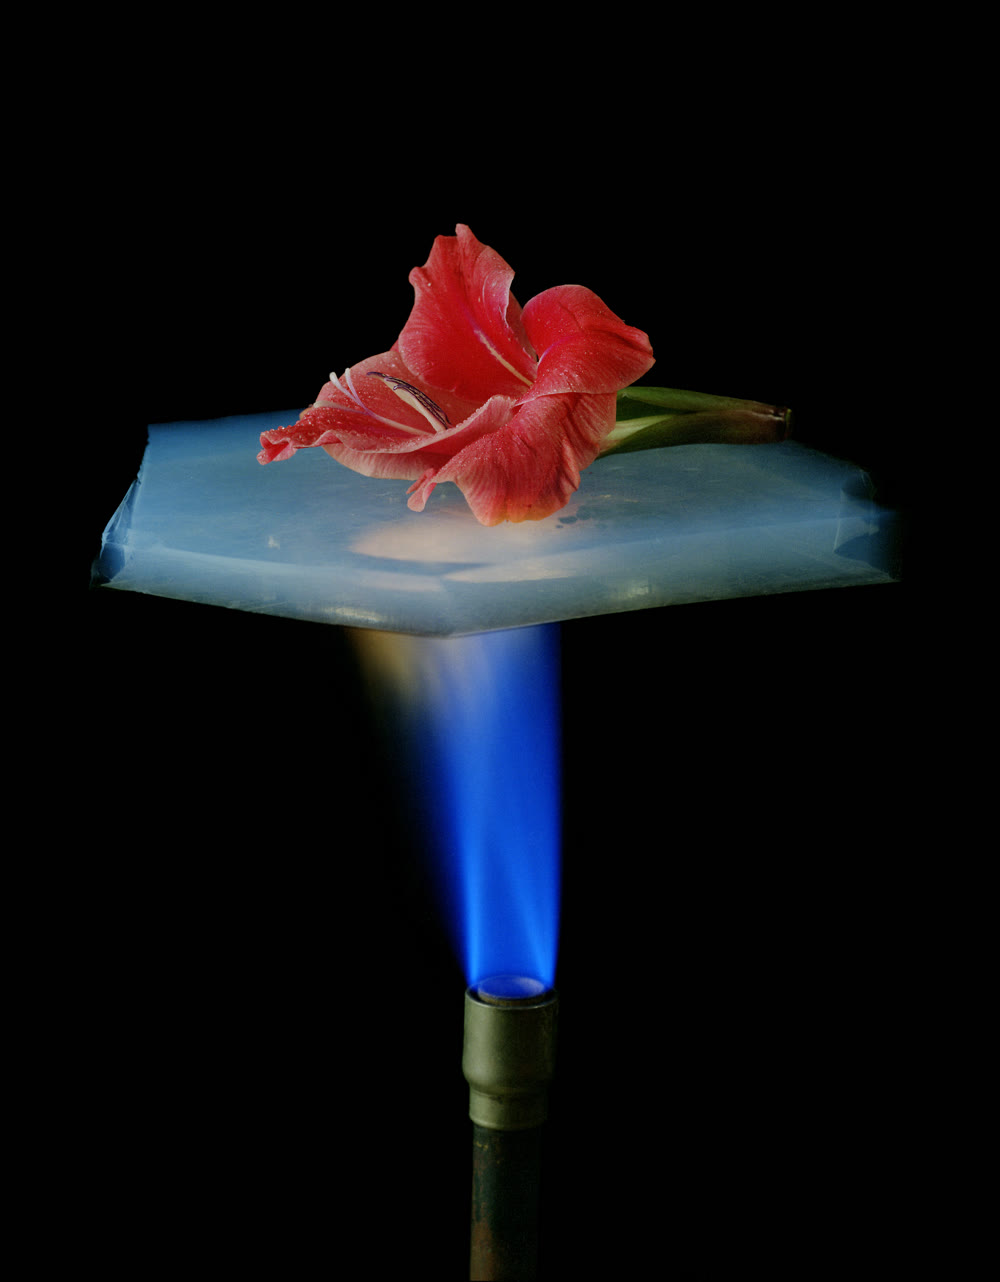
\includegraphics[width=0.38\linewidth]{images/book4/aerogel-flower.jpg}

{\small 二氧化硅气凝胶块上的花，置于燃气火焰上方：该气凝胶
是一种干燥凝胶，其中大部分为空隙，导热性极差。照片：
NASA/JPL，公有领域。}
\end{omfigure}

\section{制备路线}

\begin{definition}[陶瓷法]\label{def:b3:inorganic-materials:ceramic-method}
\emph{陶瓷法}\index{陶瓷法}通过将固体反应物
共同研磨并加热来制备固体化合物，常需数日并多次重新研磨，
温度须足够高，使离子能够在
固体中扩散。
\end{definition}

两种固体的反应发生在它们的接触处，产物在二者之间形成一层，
离子必须穿过该层方能继续迁移：最慢的步骤
是扩散，且随产物层增厚而减慢。

\begin{proposition}[抛物线型生长]\label{prop:b3:inorganic-materials:parabolic}
若产物层的生长受其间扩散限制，则其
厚度的增长满足 $x^2 = kt$。
\end{proposition}

\begin{proof}
在层的两个表面浓度固定的条件下，通过该层的通量
服从菲克定律 $J = D\Delta c/x$。产物层的增长与通量成正比：
$\dd x/\dd t = \lambda J = \lambda D\Delta c/x$，其中 $\lambda$ 为每输运一摩尔物质时产物的体积。
于是 $x\,\dd x = \lambda D\Delta c\,\dd t$，积分（由 $x = 0$ 起，$t = 0$ 时）得 $x^2 = 2\lambda D\Delta c\,t = kt$。
\end{proof}

因此颗粒尺寸加倍，反应时间即增为四倍。由此
可见需要细磨、在前驱体中达到原子尺度的混合（即分解为目标产物的
混合草酸盐或柠檬酸盐凝胶），或采用溶液法。

\begin{definition}[溶胶–凝胶法]\label{def:b3:inorganic-materials:sol-gel}
\emph{溶胶–凝胶法}\index{溶胶–凝胶法}是
以溶液中分子前驱体（通常为醇盐）的水解与缩聚制备氧化物的方法：
溶液先形成小氧化物团簇的溶胶，继而形成凝胶，即充满液体的
连续固体网络。凝胶经蒸发干燥，收缩为致密的\emph{干凝胶}\index{干凝胶}；
若在液体临界点以上干燥，
则可在无液–气界面的情况下除去液体，使凝胶保持
其体积，成为\emph{气凝胶}\index{气凝胶}。
\end{definition}

\begin{omfigure}
\setchemfig{atom sep=2.0em}
\schemestart
\chemfig{RO-Si(-[2]OR)(-[6]OR)-OR}
\+ \chemfig{H_2O}
\arrow{->[水解]}[,1.4]
\chemfig{RO-Si(-[2]OR)(-[6]OR)-OH}
\+ ROH
\schemestop
\par\bigskip
\schemestart
\chemfig{{\equiv}Si-OH}
\+
\chemfig{HO-Si{\equiv}}
\arrow{->[缩聚]}[,1.6]
\chemfig{{\equiv}Si-O-Si{\equiv}}
\+ \chemfig{H_2O}
\schemestop
\par\medskip

{\small 硅醇盐的溶胶–凝胶化学（R 为烷基，在正硅酸四乙酯中为乙基）：
水以羟基取代烷氧基，两个硅醇缩合形成硅氧桥，
反复缩合便构筑出
三维二氧化硅网络。}
\end{omfigure}

两反应合并给出完全反应的结果：
$\ce{Si(OC2H5)4 + 2H2O -> SiO2 + 4C2H5OH}$。酸催化使水解加快、
缩合减慢，生成细长链状的聚合物；碱催化则相反，
生成致密的颗粒。涂层（玻璃上的增透层）
通过将工件浸入溶胶再提拉取出制得。

\begin{definition}[水热合成]\label{def:b3:inorganic-materials:hydrothermal}
\emph{水热合成}\index{水热合成}是在高于水的正常沸点、
密闭容器内并处于自身蒸气压下，从水中使固体结晶的方法；
\emph{溶剂热合成}\index{溶剂热合成}
则是在另一种溶剂中进行同样的过程。
\end{definition}

\begin{definition}[化学气相沉积]\label{def:b3:inorganic-materials:cvd}
\emph{化学气相沉积}\index{化学气相沉积}（CVD）借助
气态前驱体在加热表面上发生反应，从而生长固体薄膜，
例如由硅烷生成硅，$\ce{SiH4 -> Si + 2H2}$，或由甲烷与氢气生成金刚石。
\end{definition}

\begin{method}[选择合成路线]\label{met:b3:inorganic-materials:route}
\begin{enumerate}
  \item 块状粉末形式的稳定难熔氧化物：
        采用陶瓷法，若混合困难则加入前驱体。
  \item 低温下得到的亚稳相、细粉或涂层：
        采用溶胶–凝胶法或沉淀反应。
  \item 仅溶于热水的物相（如石英）的大单晶，或
        以模板构筑的骨架（如沸石）：水热合成。
  \item 底物上的薄而纯的膜（如半导体层）：化学气相沉积。
\end{enumerate}
\end{method}

\begin{inthelab}[溶胶–凝胶涂层与高压釜]
将正硅酸四乙酯与乙醇、水和一滴酸搅拌，直至溶液澄清；
取一片洁净的载玻片浸入，以稳定缓慢的速率提拉，
干燥并加热后，得到薄至可呈现干涉色的二氧化硅膜。
水热合成时，将反应物放入聚四氟乙烯内衬中，
装入量不超过约三分之二，以防受热膨胀的液体充满容器，
再密封于钢制高压釜中，置于烘箱内加热；
待高压釜冷却后方可开启。
\end{inthelab}

\begin{omfigure}
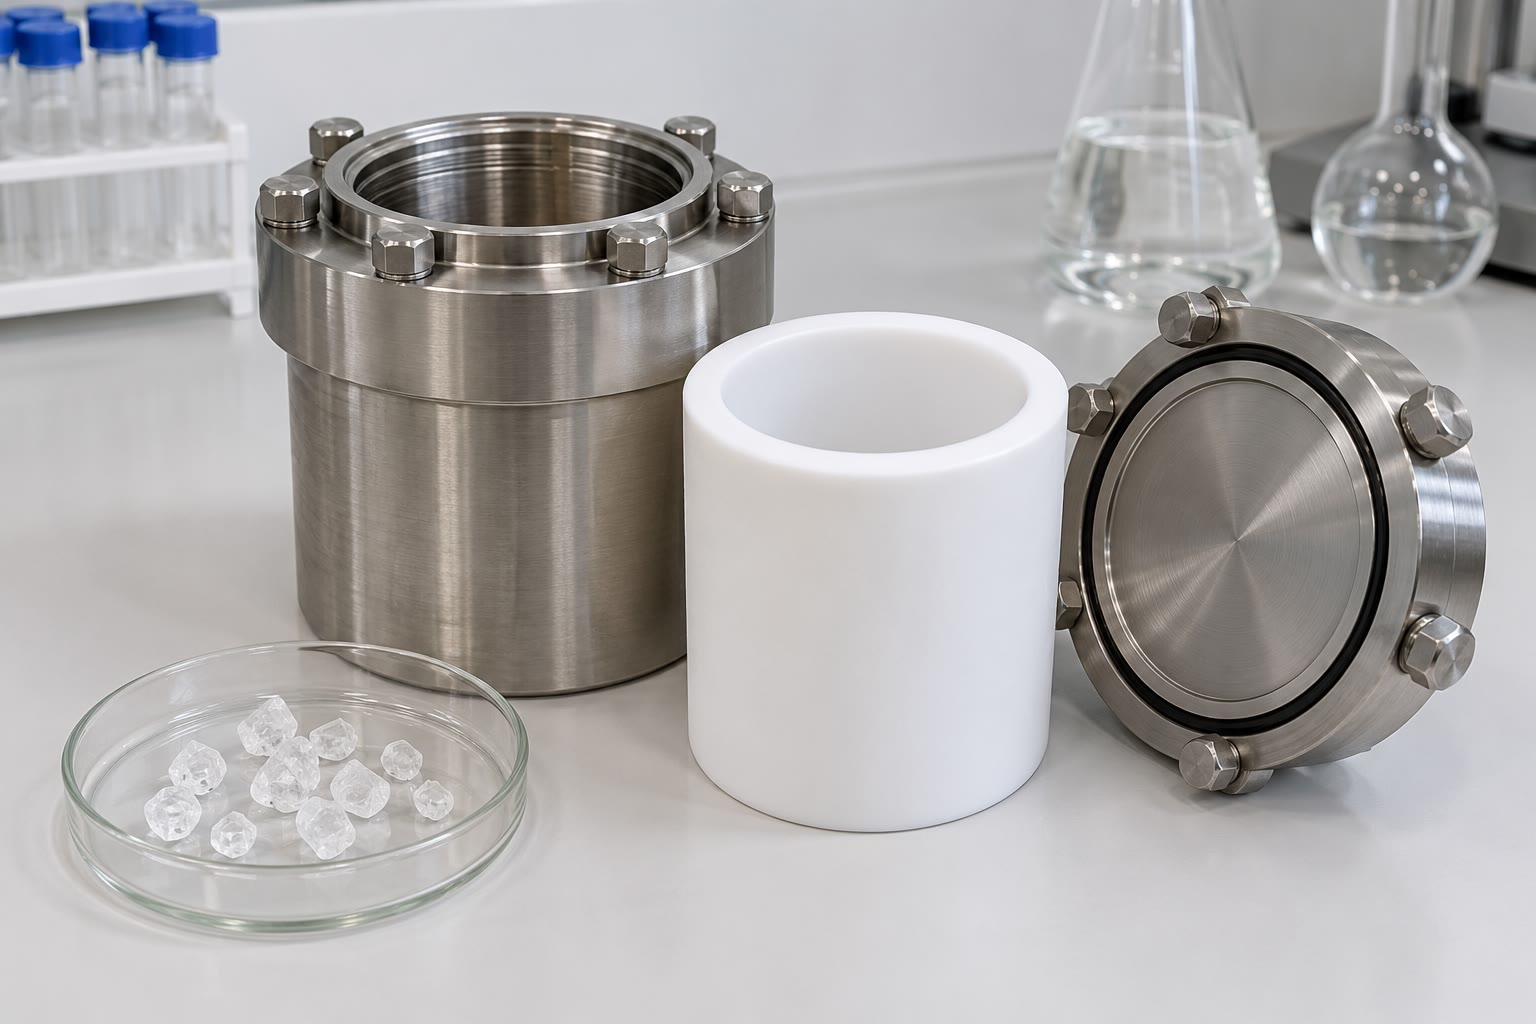
\includegraphics[width=0.5\linewidth]{images/book4/ai/b3-23-autoclave.jpg}

{\small 用于水热合成的实验室高压釜：钢制釜体，
配螺栓固定釜盖、盛放反应混合物的白色聚合物内衬，以及
其中生长出的晶体。}
\end{omfigure}

\section{陶瓷与玻璃}

\begin{definition}[陶瓷]\label{def:b3:inorganic-materials:ceramic}
称\emph{陶瓷}\index{陶瓷}为由粉末加热制成的无机非金属固体，
如氧化物、氮化物和碳化物，或黏土制品。
\end{definition}

\begin{definition}[钙钛矿结构]\label{def:b3:inorganic-materials:perovskite}
\emph{钙钛矿结构}\index{钙钛矿结构}是氧化物 $\mathrm{ABO_3}$ 的一种结构：
小的 B 阳离子位于角共享 $\mathrm{BO_6}$ 八面体的中心，
大的 A 阳离子位于其间的十二配位空隙中；
在理想立方晶胞中，B 位于体心，O 位于面心，A 位于顶点。
\emph{容忍因子}\index{容忍因子}用于衡量离子
的契合程度：
\[
  t = \frac{r_A + r_O}{\sqrt2\,(r_B + r_O)}.
\]
\end{definition}

\begin{omfigure}
\tdplotsetmaincoords{60}{100}
\begin{tikzpicture}[tdplot_main_coords, scale=1.5, font=\small,
  aA/.style={om atom, ball color=green!45!black, minimum size=7.4mm},
  aB/.style={om atom, ball color=black!35, minimum size=4.4mm},
  aOs/.style={om atom, ball color=red!80, minimum size=4.8mm}]
  \pic[transform shape] {omcubeo={2}};
  % atoms back to front for view 60/100 (depth 0.853x + 0.150y + 0.5z)
  \node[aA] at (0,0,0) {};
  \node[aA] at (0,2,0) {};
  \node[aOs] (o1) at (0,1,1) {};
  \node[aA] at (0,0,2) {};
  \node[aOs] (o2) at (1,1,0) {};
  \node[aA] at (0,2,2) {};
  \node[aOs] (o3) at (1,0,1) {};
  \node[aB] (b) at (1,1,1) {};
  \node[aOs] (o4) at (1,2,1) {};
  \node[aA] at (2,0,0) {};
  \node[aOs] (o5) at (1,1,2) {};
  \node[aA] at (2,2,0) {};
  \node[aOs] (o6) at (2,1,1) {};
  \node[aA] at (2,0,2) {};
  \node[aA] at (2,2,2) {};
  \begin{scope}[on background layer]
    \draw[omMeth!70, line width=0.6pt] (o1.center) -- (o2.center) -- (o6.center) -- (o5.center) -- cycle
      (o3.center) -- (o2.center) -- (o4.center) -- (o5.center) -- cycle
      (o1.center) -- (o3.center) -- (o6.center) -- (o4.center) -- cycle;
    \draw[bond] (b.center) -- (o1.center) (b.center) -- (o2.center) (b.center) -- (o3.center)
      (b.center) -- (o4.center) (b.center) -- (o5.center) (b.center) -- (o6.center);
  \end{scope}
  \node[anchor=west] at (2,3.35,2) {A};
  \node[anchor=west] at (2,3.35,1) {O};
  \node[anchor=west] at (2,3.35,0) {B};
  \node[aA, minimum size=4mm] at (2,3.2,2) {};
  \node[aOs, minimum size=3.2mm] at (2,3.2,1) {};
  \node[aB, minimum size=3mm] at (2,3.2,0) {};
\end{tikzpicture}

{\small 立方钙钛矿晶胞 $\mathrm{ABO_3}$：B 阳离子（灰色）位于
由面心六个氧离子构成的八面体中心（绿色棱边），A 阳离子位于顶点。
每个顶点的 A 离子被八个晶胞共享，每个氧离子被两个晶胞共享，
因此每个晶胞含一个 A、一个 B 和三个 O。}
\end{omfigure}

\begin{proposition}[理想容忍因子]\label{prop:b3:inorganic-materials:tolerance}
在理想立方钙钛矿中，离子沿 B--O 和 A--O 方向相互接触，
则 $t = 1$。
\end{proposition}

\begin{proof}
棱长为 $a$ 时，B 位于中心，O 位于面心，二者相距 $a/2$：$r_B + r_O = a/2$。
A 位于顶点，O 位于相邻面的面心，二者相距半个面对角线：
$r_A + r_O = a\sqrt2/2$。两式相除得 $(r_A + r_O)/(r_B + r_O) = \sqrt2$，故 $t = 1$。
\end{proof}

当 $t$ 略小于 1 时，A 离子相对其空隙过小，
八面体发生倾斜以围拢它，从而降低对称性；当 $t$ 大于 1 时，
B 离子相对其八面体过小，可偏离中心移动。

\begin{definition}[铁电体]\label{def:b3:inorganic-materials:ferroelectric}
称\emph{铁电体}\index{铁电体}为一种具有自发
电极化、且能被外电场反转的晶体。
\end{definition}

% ledger: rion:Ba2+XII, rion:Ti4+VI, rion:O2-VI
钛酸钡是典型例子：$r(\ce{Ba^2+}) = \qty{161}{pm}$（十二配位），
$r(\ce{Ti^4+}) = \qty{60.5}{pm}$，$r(\ce{O^2-}) = \qty{140}{pm}$，$t = 1.06$。低于某一转变温度时，
钛离子偏离中心，同一畴内的离子均沿同一方向移动，
晶体产生极化；转变温度附近的介电常数极大，
因此钛酸钡成为大多数陶瓷电容器所用的电介质。

\begin{definition}[氧化物玻璃]\label{def:b3:inorganic-materials:glass}
称\emph{氧化物玻璃}\index{氧化物玻璃}为一种非晶态氧化物固体，
由熔体冷却而成，冷却时不发生结晶。其\emph{网络
形成体}\index{网络形成体}（$\ce{SiO2}$、$\ce{B2O3}$、$\ce{P2O5}$）构成由共角多面体连接的连续网络；
其\emph{网络修饰体}\index{网络修饰体}
（$\ce{Na2O}$、$\ce{CaO}$）会打断该网络中的桥键，每加入一个氧离子，
就使一个桥氧变为两个非桥氧，阳离子位于
空穴中。
\end{definition}

\begin{omfigure}
\begin{tikzpicture}
\begin{axis}[name=c, width=0.5\linewidth, axis equal image, hide axis, xmin=-1.2, xmax=12.6, ymin=-1.2, ymax=8.7]
\addplot[quiver={u=\thisrow{u}, v=\thisrow{v}}, -, black!60, line width=0.6pt] table {figdata/out/bachelor-3-glass-network-crystal-bonds.dat};
\addplot[only marks, mark=*, mark size=2.2pt, omDef] table {figdata/out/bachelor-3-glass-network-crystal-T.dat};
\addplot[only marks, mark=*, mark size=1.3pt, omThm, mark options={fill=white}] table {figdata/out/bachelor-3-glass-network-crystal-O.dat};
\end{axis}
\begin{axis}[at={(c.east)}, anchor=west, xshift=0.2cm, width=0.5\linewidth, axis equal image, hide axis, xmin=-1.2, xmax=12.6, ymin=-1.2, ymax=8.7]
\addplot[quiver={u=\thisrow{u}, v=\thisrow{v}}, -, black!60, line width=0.6pt] table {figdata/out/bachelor-3-glass-network-glass-bonds.dat};
\addplot[only marks, mark=*, mark size=2.2pt, omDef] table {figdata/out/bachelor-3-glass-network-glass-T.dat};
\addplot[only marks, mark=*, mark size=1.3pt, omThm, mark options={fill=white}] table {figdata/out/bachelor-3-glass-network-glass-O.dat};
\addplot[only marks, mark=*, mark size=1.5pt, omThm] table {figdata/out/bachelor-3-glass-network-glass-NBO.dat};
\addplot[only marks, mark=*, mark size=2.6pt, omProp] table {figdata/out/bachelor-3-glass-network-glass-Na.dat};
\end{axis}
\end{tikzpicture}

{\small 同一组成的晶体与玻璃的二维示意图（
蓝色：三配位形成体；空心红圈：桥氧）。
左图中，晶体重复同一个环。右图为玻璃：每个形成体仍有三个氧，
且距离几乎相同，但环由五元、六元或七元构成，且无重复规律；
两处修饰体打断了桥键，留下两个非桥氧（实心红点）
及位于空穴中的阳离子（橙色）。
模型网络，由弹簧弛豫得到。}
\end{omfigure}

1932 年，扎卡里亚森提出：当氧化物的阳离子周围仅有少数（三个或四个）氧时，
每个氧至多连接两个阳离子，且多面体只共享顶角、不共棱或共面，
则无规网络所需的能量并不比晶体多，因此氧化物易于形成玻璃。
窗玻璃是加入氧化钠与氧化钙作修饰体的二氧化硅，二者可降低熔点。手机
的增韧盖板玻璃用熔融硝酸钾浸泡处理：
较大的 $\ce{K+}$ 离子取代表层中的 $\ce{Na+}$ 离子，
由于排列拥挤，使表层处于压应力之下，
从而裂纹不易张开。

\section{多孔固体：沸石与框架结构}

\begin{definition}[沸石]\label{def:b3:inorganic-materials:zeolite}
称\emph{沸石}\index{沸石}为一种晶态铝硅酸盐，其
由共角的 $\ce{SiO4}$ 与 $\ce{AlO4}$ 四面体构成的骨架围成尺寸与分子相当的笼和孔道，
笼和孔道内含可交换的阳离子与水。
称\emph{分子筛}\index{分子筛}为一种依分子尺寸允许分子通过的多孔固体；
\emph{择形性}\index{择形性}是指借助孔道的大小与形状，
对反应进行的控制，
反应即在这些孔道中进行。
\end{definition}

每个 $\ce{AlO4}$ 四面体比 $\ce{SiO4}$ 四面体多带一个负电荷
（以三价铝代替四价硅）；笼中的阳离子 $\ce{Na+}$ 或 $\ce{Ca^2+}$ 与之平衡，
并可被交换。

\begin{proposition}[洛文斯坦规则]\label{prop:b3:inorganic-materials:lowenstein}
在沸石骨架中，两个 $\ce{AlO4}$ 四面体从不共用一个氧，即不存在 Al--O--Al 连接
（对所有已知铝硅酸盐骨架的观察结果）。由此可得，
沸石的硅铝比 Si/Al 至少为 1。
\end{proposition}

\begin{proof}[推论的证明]
由上述规则，每个铝有四个氧，且每个氧都与一个硅共用，
故有 $4N_{\mathrm{Al}}$ 个 Al--O--Si 连接。每个硅只有四个氧，因此至多参与四个这样的连接：
$4N_{\mathrm{Al}} \le 4N_{\mathrm{Si}}$，即 $N_{\mathrm{Si}}/N_{\mathrm{Al}} \ge 1$。取等号时，每个硅都须有四个铝邻居：
硅与铝交替排列。
\end{proof}

\begin{omfigure}
\tdplotsetmaincoords{55}{135}
\begin{tikzpicture}[tdplot_main_coords, scale=0.85, font=\small, baseline=(current bounding box.center),
  tSi/.style={circle, inner sep=0pt, minimum size=2.6mm, draw=black!70, fill=omDef!80},
  tAl/.style={circle, inner sep=0pt, minimum size=2.6mm, draw=black!70, fill=omProp!80}]
  % edges of a truncated octahedron (vertices: permutations of (0, +-1, +-2));
  % hidden edges (both faces facing away for this view) dashed
  \foreach \a/\b/\c/\d/\e/\f in {-2/-1/0/-2/0/-1, -2/-1/0/-2/0/1, -2/-1/0/-1/-2/0, -2/0/-1/-2/1/0, -2/0/-1/-1/0/-2, -1/-2/0/0/-2/-1, -1/-2/0/0/-2/1, -1/0/-2/0/-1/-2, -1/0/-2/0/1/-2, 0/-2/-1/0/-1/-2, 0/-2/-1/1/-2/0, 0/-1/-2/1/0/-2}
    \draw[black!40, dashed] (\a,\b,\c) -- (\d,\e,\f);
  \foreach \a/\b/\c/\d/\e/\f in {-2/0/1/-2/1/0, -2/0/1/-1/0/2, -2/1/0/-1/2/0, -1/0/2/0/-1/2, -1/0/2/0/1/2, -1/2/0/0/2/-1, -1/2/0/0/2/1, 0/-2/1/0/-1/2, 0/-2/1/1/-2/0, 0/-1/2/1/0/2, 0/1/-2/0/2/-1, 0/1/-2/1/0/-2, 0/1/2/0/2/1, 0/1/2/1/0/2, 0/2/-1/1/2/0, 0/2/1/1/2/0, 1/-2/0/2/-1/0, 1/0/-2/2/0/-1, 1/0/2/2/0/1, 1/2/0/2/1/0, 2/-1/0/2/0/-1, 2/-1/0/2/0/1, 2/0/-1/2/1/0, 2/0/1/2/1/0}
    \draw[black!75, line width=0.7pt] (\a,\b,\c) -- (\d,\e,\f);
  % T atoms back to front; hidden ones paler
  \foreach \x/\y/\z/\k/\v in {-2/-1/0/Si/0, -1/-2/0/Al/0, -2/0/-1/Al/0, 0/-2/-1/Si/0, -1/0/-2/Si/0, 0/-1/-2/Al/0, -2/0/1/Al/1, 0/-2/1/Si/1, -2/1/0/Si/1, 1/-2/0/Al/1, 0/1/-2/Al/1, 1/0/-2/Si/1, -1/0/2/Si/1, 0/-1/2/Al/1, -1/2/0/Al/1, 2/-1/0/Si/1, 0/2/-1/Si/1, 2/0/-1/Al/1, 0/1/2/Al/1, 1/0/2/Si/1, 0/2/1/Si/1, 2/0/1/Al/1, 1/2/0/Al/1, 2/1/0/Si/1}
    \node[t\k, opacity=0.35+0.65*\v] at (\x,\y,\z) {};
\end{tikzpicture}
\hspace{1.2cm}
\begin{tikzpicture}[font=\small, scale=0.8, baseline=(current bounding box.center)]
  \foreach \i in {0,1,2} \foreach \j in {0,1,2} {
    \fill[omDef!70] ($(2.2*\i,2.2*\j)+(-0.28,-0.28)$) rectangle +(0.56,0.56);
  }
  \foreach \i in {0,1} \foreach \j in {0,1,2} {
    \draw[black!70, line width=0.8pt] (2.2*\i+0.28,2.2*\j) -- (2.2*\i+0.75,2.2*\j);
    \draw[black!70, line width=0.8pt] (2.2*\i+1.45,2.2*\j) -- (2.2*\i+1.92,2.2*\j);
    \node[draw=black!70, regular polygon, regular polygon sides=6, minimum size=5.6mm, inner sep=0pt] at (2.2*\i+1.1,2.2*\j) {};
  }
  \foreach \i in {0,1,2} \foreach \j in {0,1} {
    \draw[black!70, line width=0.8pt] (2.2*\i,2.2*\j+0.28) -- (2.2*\i,2.2*\j+0.75);
    \draw[black!70, line width=0.8pt] (2.2*\i,2.2*\j+1.45) -- (2.2*\i,2.2*\j+1.92);
    \node[draw=black!70, regular polygon, regular polygon sides=6, minimum size=5.6mm, inner sep=0pt] at (2.2*\i,2.2*\j+1.1) {};
  }
  \node[font=\scriptsize, align=center] at (1.1,-0.85) {$\ce{Zn4O}$ 节点 $+$ 对苯二甲酸连接体};
\end{tikzpicture}

{\small 左：方钠石笼，即沸石 A 的构筑单元，每个顶角为一个四面体原子
（氧原子位于各棱中点，未画出）；硅（蓝色）与铝（橙色）交替排列，
符合洛温斯坦规则在 Si/Al = 1 时的要求。右：
金属–有机框架的一层（示意）：
$\ce{Zn4O}$ 簇（方块）经苯-1,4-二羧酸根连接体（环）
相连，形成具有大孔道的立方网格。}
\end{omfigure}

\begin{method}[沸石的化学式与交换容量]\label{met:b3:inorganic-materials:zeolite-formula}
\begin{enumerate}
  \item 将骨架写作 $\mathrm{[(AlO_2)_x(SiO_2)_y]^{x-}}$：Si/Al $= y/x$。
  \item 骨架电荷 $-x$ 由阳离子平衡：$x$ 个一价阳离子或 $x/2$
        个二价阳离子。
  \item 交换容量是每克可交换电荷的量：
        一价阳离子为 $x/M$ 摩尔，二价阳离子为 $x/2M$ 摩尔，其中 $M$ 为
        按称量时的形式计算的化学式摩尔质量（无水或含水）。
\end{enumerate}
\end{method}

\begin{proposition}[交换容量]\label{prop:b3:inorganic-materials:exchange-capacity}
沸石对电荷为 $z$ 的阳离子的容量为每克 $x/(zM)$ 摩尔，
其中 $x$ 为摩尔质量为 $M$ 的化学式中铝原子的个数。
\end{proposition}

\begin{proof}
每个铝原子为骨架提供一个负电荷，电中性要求
$x$ 个单位的正电荷，且均可交换，因此
每个化学式单元含 $x/z$ 个电荷为 $z$ 的阳离子，即每质量 $M$。
\end{proof}

% ledger: iza:LTA.window, iza:MFI.channels
沸石 A 的孔口由八个四面体构成，直径 \qty{0.41}{nm}：水和小
离子可以通过，支链分子则不能。ZSM-5 有两组通道，每组由十个
四面体构成，孔径约 0.51 至 \qty{0.56}{nm}：在甲醇转化或
甲苯烷基化中，细长的对位-二甲苯扩散出去的速度远快于它的
邻位-与间位-异构体，后者留在孔内并发生异构化。这就是
择形性。

\begin{definition}[金属–有机框架]\label{def:b3:inorganic-materials:mof}
称\emph{金属–有机框架}\index{金属–有机框架}（MOF）为一种
由金属离子或金属簇经多齿有机连接体相连而成的晶态固体，
形成多孔网络。\emph{次级构筑
单元}\index{次级构筑单元}是金属簇及其配位基团，
在网络中视为一个节点；\emph{网格
合成}\index{网格合成}是通过
选取具有给定几何形状的节点与连接体，使其组装成指定网络的框架设计。
\end{definition}

% ledger: cod:MOF5.formula, cod:MOF5.a
在 MOF-5 中，带六个羧酸根基团的 $\ce{Zn4O}$ 簇构成八面体节点，
苯-1,4-二羧酸根连接体沿立方网格的棱将它们相连，
网格，含八个节点的晶胞中 $a = \qty{25.82}{\angstrom}$。用更长的连接体替换
原连接体，网格保持不变而孔道增大，这正是网格合成的思想。此类
框架的比表面积达每克数千平方米，并
被研究用于储存氢气和甲烷，以及捕获二氧化碳。

\begin{definition}[孔径]\label{def:b3:inorganic-materials:pores}
% ledger: pore:micro, pore:macro
按约定，\emph{微孔}\index{微孔}的孔径小于 \qty{2}{nm}，
\emph{介孔}\index{介孔}的孔径介于 2 至 \qty{50}{nm} 之间，而
\emph{大孔}\index{大孔}的孔径大于 \qty{50}{nm}。
\end{definition}

沸石和大多数 MOF 为微孔材料；硅胶和气凝胶则为介孔材料。

\section{纳米颗粒}

\begin{definition}[纳米材料]\label{def:b3:inorganic-materials:nano}
称\emph{纳米材料}\index{纳米材料}为至少有一维
尺寸约在 1 与 \qty{100}{nm} 之间的材料；\emph{纳米颗粒}\index{纳米颗粒}则
三维尺寸均在此范围内。
\end{definition}

\begin{proposition}[幻数团簇]\label{prop:b3:inorganic-materials:magic}
由一个中心原子和 $n$ 个完整壳层构成的立方八面体团簇具有
\[
  N(n) = \frac{10n^3 + 15n^2 + 11n + 3}{3}
\]
个原子，其中 $10n^2 + 2$ 个位于表面：13、55、147、309、\dots
\end{proposition}

\begin{proof}
立方八面体的第 $k$ 个壳层有 12 个顶点、24 条棱，每条棱上
有 $k - 1$ 个内部原子，8 个三角面各含 $(k - 1)(k - 2)/2$ 个内部原子，6
个正方形面各含 $(k - 1)^2$ 个原子，共计 $12 + 24(k - 1) + 4(k - 1)(k - 2) + 6(k - 1)^2 = 10k^2 + 2$。于是
$N(n) = 1 + \sum_{k=1}^{n}(10k^2 + 2) = 1 + \frac{10n(n + 1)(2n + 1)}{6} + 2n$，展开即得上式；
最外壳层含 $10n^2 + 2$ 个原子，构成表面。
\end{proof}

\begin{omfigure}
\begin{tikzpicture}
\begin{axis}[name=a, width=0.47\linewidth, height=5.4cm, xmin=0, xmax=18, ymin=0, ymax=1,
  axis lines=left, xlabel={直径 / \unit{nm}}, ylabel={表面原子分数},
  tick label style={font=\scriptsize}, label style={font=\small}]
\addplot[omDef, thick, mark=*, mark size=1pt] table[x=diam_nm, y=fsurf] {figdata/out/bachelor-3-nanoparticle-size.dat};
\end{axis}
\begin{axis}[at={(a.east)}, anchor=west, xshift=1.5cm, width=0.47\linewidth, height=5.4cm,
  xmin=0.8, xmax=6, ymin=0, ymax=3, axis lines=left,
  xlabel={半径 $R$ / \unit{nm}}, ylabel={限域能 / \unit{eV}},
  tick label style={font=\scriptsize}, label style={font=\small}]
\addplot[omThm, thick] table[x=R_nm, y=dE_eV] {figdata/out/bachelor-3-nanoparticle-size-b.dat};
\end{axis}
\end{tikzpicture}

{\small 左：立方八面体金团簇中表面原子所占分数
随直径的变化：直径小于约
\qty{3}{nm} 时超过一半，\qty{8}{nm} 时仍约占五分之一。右：
球形量子点中电子–空穴对的限域能（模型约化质量 $0.10\,m_e$），
它使带隙增大，并随 $1/R^2$ 下降。}
\end{omfigure}

由于大部分原子位于表面，那里的近邻较少，
纳米颗粒的熔点低于块状金属，
反应活性更高，也可能是更好的催化剂：块状金不活泼，金
颗粒（直径仅几纳米）在室温下即可氧化一氧化碳。

\begin{definition}[量子点]\label{def:b3:inorganic-materials:quantum-dot}
称\emph{量子点}\index{量子点}为半导体纳米晶，其尺寸足够小，
使电子与空穴的限域作用令其带隙
高于块状固体的带隙。
\end{definition}

\begin{theorem}[球内限域]\label{thm:b3:inorganic-materials:quantum-dot}
质量为 $m$ 的粒子被无限高势壁限制在半径为 $R$ 的球形区域内，
其基态能量为 $E = \hbar^2\pi^2/(2mR^2) = h^2/(8mR^2)$，波函数为 $\psi \propto \sin(\pi r/R)/r$。
\end{theorem}

\begin{proof}
对球对称态 $\psi(r) = u(r)/r$，拉普拉斯算子给出
$\nabla^2\psi = u''/r$，因此球内薛定谔方程化为 $-\frac{\hbar^2}{2m}u'' = Eu$，与直线上粒子的方程相同。
在球心处 $\psi$ 有限的解满足 $u(0) = 0$，此时 $u = \sin(kr)$，且 $E = \hbar^2k^2/2m$。
势壁要求 $u(R) = 0$，故基态时 $kR = \pi$，于是 $E = \hbar^2\pi^2/(2mR^2)$。
\end{proof}

在量子点中，电子和空穴都受到限域，最低激发态的能量
近似为 $E_g + h^2/(8\mu R^2)$，其中 $\mu$ 为二者的约化质量
（两者间的库仑吸引使之略有降低）。半径减半时
限域能变为原来的四倍：直径几纳米的硒化镉量子点
仅凭尺寸即可发出红、绿或蓝光，被用作
显示器中的发光体。

\begin{definition}[表面等离子体共振]\label{def:b3:inorganic-materials:plasmon}
称\emph{表面等离子体共振}\index{表面等离子体共振}为
由光驱动的金属纳米颗粒中导电电子的集体振荡；
它给出强吸收带，其波长取决于
金属种类、颗粒的大小与形状及其周围环境。
\end{definition}

直径几十纳米的金纳米颗粒吸收绿光，
在玻璃或胶体中呈宝石红色；颗粒聚集时，吸收带向长波方向移动，
颜色变为蓝色。这是许多快速检测的基础，其中
表面包覆抗体的金胶体会聚集成一条有色条带。

\section{碳纳米材料}

\begin{definition}[碳纳米材料]\label{def:b3:inorganic-materials:carbon}
称\emph{富勒烯}\index{富勒烯}为由碳原子构成的封闭笼状分子，
每个碳原子与另外三个原子成键，由五元环和六元环组成，如
二十面体的 $\ce{C60}$。称\emph{碳纳米管}\index{碳纳米管}为
由石墨片卷成的无缝圆柱体，直径约一纳米。
\emph{石墨烯}\index{石墨烯}是单层石墨，厚度仅一个原子。
\end{definition}

\begin{proposition}[十二个五边形]\label{prop:b3:inorganic-materials:euler}
任何富勒烯恰好有十二个五边形，
与六边形的个数无关。
\end{proposition}

\begin{proof}
封闭笼状结构是一个多面体，欧拉公式 $V - E + F = 2$ 成立。每个原子有
三条键，每条键连接两个原子：$2E = 3V$。设有 $p$ 个五边形、$h$ 个六边形，
按面计数棱，得 $2E = 5p + 6h$，且 $F = p + h$。于是 $V = 2E/3$，欧拉公式
写为 $-E/3 + p + h = 2$，即 $-(5p + 6h)/6 + p + h = 2$，从而 $p/6 = 2$，$p = 12$。
\end{proof}

\begin{omfigure}
\begin{tikzpicture}[scale=0.62, font=\small]
  \def\hexd{0.6}
  \begin{scope}
    \clip (-0.4,-0.5) rectangle (9.6,5.2);
    \foreach \i in {-3,...,10} \foreach \j in {-1,...,6} {
      \pgfmathsetmacro\cx{1.7320508*\hexd*(\i + 0.5*\j)}
      \pgfmathsetmacro\cy{1.5*\hexd*\j}
      \draw[black!45] ({\cx+\hexd*cos(30)},{\cy+\hexd*sin(30)})
        \foreach \k in {90,150,...,390} { -- ({\cx+\hexd*cos(\k)},{\cy+\hexd*sin(\k)}) };
    }
  \end{scope}
  \draw[->, thick, omDef] (0,0) -- ({1.7320508*\hexd},0) node[below right, font=\scriptsize, fill=white, inner sep=1pt] {$\mathbf a_1$};
  \draw[->, thick, omDef] (0,0) -- ({1.7320508*\hexd*0.5},{1.5*\hexd}) node[left, font=\scriptsize, fill=white, inner sep=1pt] {$\mathbf a_2$};
  \draw[->, very thick, omThm] (0,0) -- ({1.7320508*\hexd*(4+0.5*2)},{1.5*\hexd*2}) node[above right, font=\scriptsize, fill=white, inner sep=1pt] {$\mathbf C_h = 4\mathbf a_1 + 2\mathbf a_2$};
  \draw[dashed, omMeth, thick] (0,0) -- ({1.7320508*\hexd*9},0) node[right, font=\scriptsize] {锯齿形 $(n, 0)$};
  \draw[dashed, omProp, thick] (0,0) -- ({1.7320508*\hexd*5*1.5},{1.5*\hexd*5}) node[below right, font=\scriptsize, fill=white, inner sep=1pt] {扶手椅型 $(n, n)$};
\end{tikzpicture}

{\small 石墨烯片与纳米管的手性矢量：卷起片层，使
$\mathbf C_h = n\mathbf a_1 + m\mathbf a_2$ 的端点与其起点重合，即得 $(n, m)$ 管，此处为 $(4, 2)$。
沿 $\mathbf a_1$ 方向，$(n, 0)$ 管的管口为锯齿形；沿 $\mathbf a_1 + \mathbf a_2$ 方向（夹角 30°），$(n, n)$
管的管口为扶手椅型。}
\end{omfigure}

\begin{proposition}[金属性与半导体性纳米管]\label{prop:b3:inorganic-materials:nanotube}
单壁碳纳米管 $(n, m)$ 在 $n - m$ 为 3 的倍数时为金属性的，
否则为半导体。\admitted
\end{proposition}

因此，所有可能的管中有三分之一为金属性，其中包括每一根
扶手椅型管；其余管的带隙随直径增大而减小。石墨烯本身
完全没有带隙：价带与导带仅在一些孤立点上相接，其
电子的运动仿佛没有质量。

\begin{safety}{\ghs[0.62cm]{GHS02}\ghs[0.62cm]{GHS07}\ghs[0.62cm]{GHS08}}
% ledger: ghs4:TEOS
原硅酸四乙酯：易燃液体和蒸气，吸入有害，
对眼睛和呼吸道有刺激性；应在通风橱中操作。纳米粉末：最细的
颗粒可深入肺部，许多尚未完成危险性分类；
应在密闭装置中称量和操作，或制成悬浮液，切勿
以散落粉尘的形式在敞开空气中操作。
\end{safety}

\begin{omfigure}
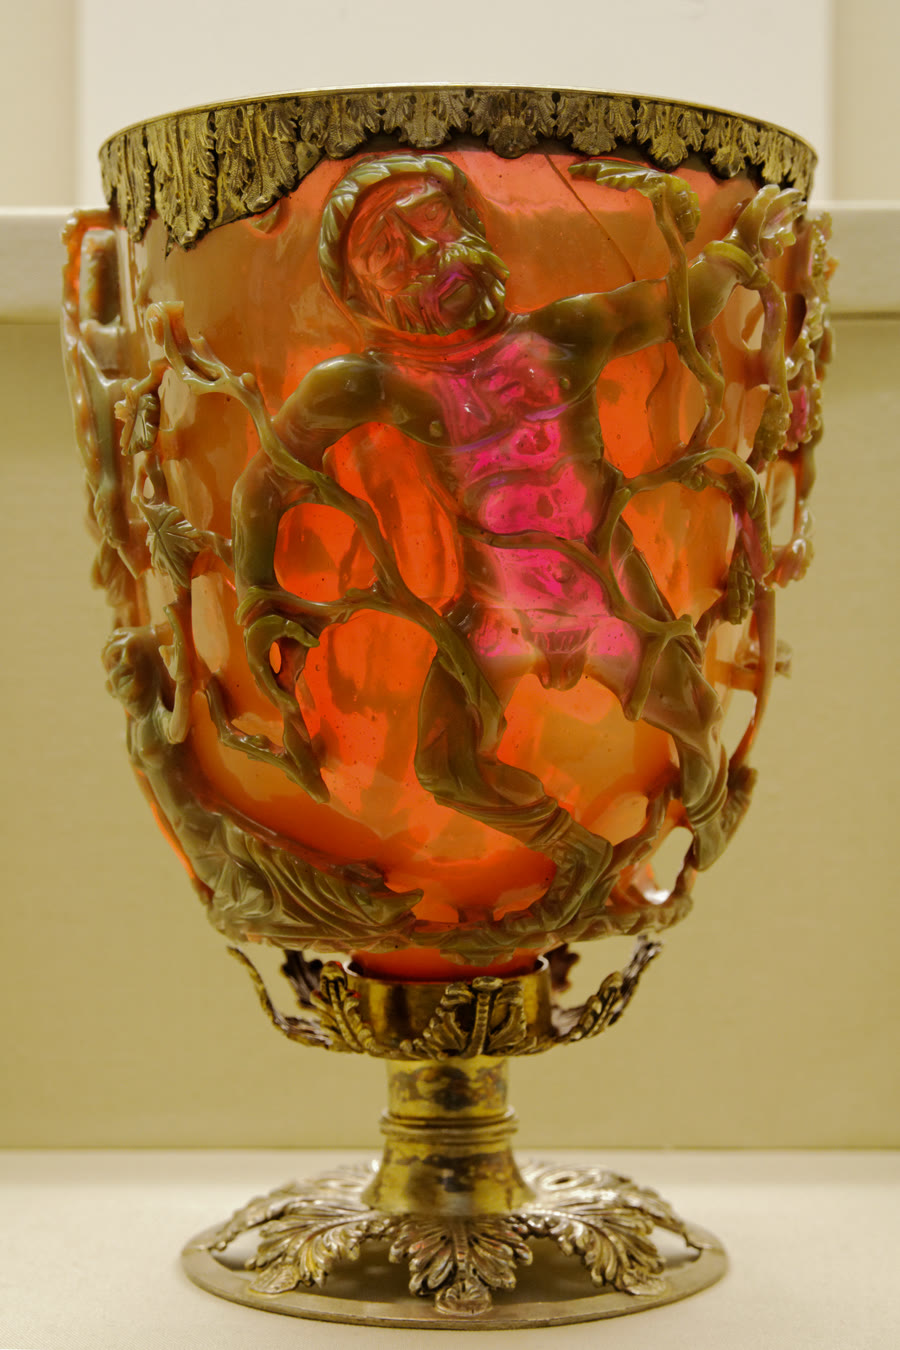
\includegraphics[width=0.32\linewidth]{images/book4/lycurgus-cup.jpg}

{\small 莱库古斯杯，一件四世纪的罗马玻璃器，从内部照亮：
它在反射光下呈绿色，在透射光下呈红色，这一效应源于玻璃中的
金–银纳米颗粒。照片：Marie-Lan Nguyen，CC BY
2.5.}
\end{omfigure}

\begin{history}[纳米颗粒之名出现之前，以及一只碳“足球”]
玻璃工匠早在人们弄清原因之前，就已用金把玻璃染成红色；
莱库古斯杯最能体现这一效应。法拉第于 1850 年代制得金胶体，
并发现其颜色来自尺寸小到肉眼无法分辨的颗粒。
1985 年，哈罗德·克罗托、罗伯特·柯尔和理查德·斯莫利用激光使石墨气化，
发现由六十个碳原子组成的团簇异常稳定，
并提出了由十二个五边形与二十个六边形构成的封闭笼状结构；
他们因此荣获 1996 年诺贝尔化学奖。
\end{history}

\section{练习}

\begin{exercise}[$\star$]\label{exo:b3:inorganic-materials:1}
两固体之间的产物层经 \qty{10}{h} 后厚度为 \qty{2.0}{\micro\metre}，
若其生长服从抛物线规律，则厚度达到 \qty{6.0}{\micro\metre} 需要多长时间？
\end{exercise}

\begin{exercise}[$\star$]\label{exo:b3:inorganic-materials:2}
写出原硅酸四乙酯水解为硅酸的反应、
两个硅酸分子缩合的反应，以及
生成二氧化硅的总反应。
\end{exercise}

\begin{exercise}[$\star$]\label{exo:b3:inorganic-materials:3}
判断 $\ce{SiO2}$、$\ce{B2O3}$、$\ce{Na2O}$ 和 $\ce{CaO}$ 各属于网络形成体还是网络修饰体，并说明
$\ce{Na2O}$ 对二氧化硅网络起什么作用。
\end{exercise}

\begin{exercise}[$\star$]\label{exo:b3:inorganic-materials:4}
$\ce{C70}$ 有多少个五边形和六边形？有多少根键？
\end{exercise}

\begin{exercise}[$\star\star$]\label{exo:b3:inorganic-materials:5}
% ledger: rion:Sr2+XII, rion:Ca2+XII, rion:Ba2+XII, rion:Ti4+VI, rion:O2-VI
计算 $\ce{SrTiO3}$、$\ce{BaTiO3}$ 和 $\ce{CaTiO3}$ 的容忍因子，
取 $\ce{Sr^2+}$（\qty{144}{pm}）、$\ce{Ba^2+}$（\qty{161}{pm}）和 $\ce{Ca^2+}$（\qty{134}{pm}）的十二配位半径，$r(\ce{Ti^4+}) = \qty{60.5}{pm}$，$r(\ce{O^2-}) = \qty{140}{pm}$。
它们预测了什么？
\end{exercise}

\begin{exercise}[$\star\star$]\label{exo:b3:inorganic-materials:6}
某沸石 X 的无水化学式为 $\mathrm{Na_{86}[(AlO_2)_{86}(SiO_2)_{106}]}$（题中数据）。
求 Si/Al 比，以及其对 $\ce{Ca^2+}$ 的交换容量（以毫摩尔每克计）。
\end{exercise}

\begin{exercise}[$\star\star$]\label{exo:b3:inorganic-materials:7}
% ledger: lat:Au
金为面心立方结构，$a = \qty{407.8}{pm}$。估算一个
直径约为 \qty{5}{nm} 的立方八面体金颗粒的壳层数、原子数以及
其表面的原子比例。
\end{exercise}

\begin{exercise}[$\star\star$]\label{exo:b3:inorganic-materials:8}
某半导体的体相带隙为 \qty{1.74}{eV}，电子与空穴的约化质量
为 $0.10\,m_e$（题中数据）。估算由
半径分别为 2.0 和 \qty{3.0}{nm} 的量子点发出的光的颜色，忽略库仑吸引。
\end{exercise}

\begin{exercise}[$\star\star$]\label{exo:b3:inorganic-materials:9}
判断纳米管 $(10, 10)$、$(10, 0)$、$(9, 0)$ 和 $(12, 8)$ 是金属性的还是半导体性的？哪些是
扶手椅型，哪些是锯齿型？
\end{exercise}

\begin{exercise}[$\star\star\star$]\label{exo:b3:inorganic-materials:10}
% ledger: cod:MOF5.formula, cod:MOF5.a, cod:MOF5.Z
MOF-5，$\mathrm{Zn_4O(C_8H_4O_4)_3}$，属立方晶系，$a = \qty{25.82}{\angstrom}$，每个晶胞含 8 个化学式单元。
计算其密度。若 1 克该材料的比表面积为 $\qty{3000}{m^2}$（题中数据），
则其总表面积相当于多少块 $\qty{105}{m} \times \qty{68}{m}$ 的足球场？
\end{exercise}

\begin{exercise}[$\star\star\star$]\label{exo:b3:inorganic-materials:11}
利用\cref{prop:b3:inorganic-materials:magic}给出的壳层数，证明
立方八面体团簇的表面比例趋于 $3/n$（$n$ 很大时），
并将 $n = 8$ 时的结果与精确比例进行比较。
\end{exercise}

\begin{exercise}[$\star\star\star$]\label{exo:b3:inorganic-materials:12}
每个原子成三根键的封闭碳笼含有 $p$ 个五边形、$h$ 个六边形
和 $s$ 个七边形。证明 $p - s = 12$。
\end{exercise}

\section{周末问题：用 A 型沸石软化水}

\begin{problem}[{周末问题——用 A 型沸石软化水：化学式与勒文斯坦规则、
理论交换容量、一次洗涤所需的沸石量，以及
允许钙离子进入、阻止洗涤剂通过的
孔口}]
\label{pb:b3:inorganic-materials:1}
% ledger: iza:LTA.formula, iza:LTA.window, aw:Na, aw:Al, aw:Si, aw:O, aw:H, aw:Ca, aw:C, rion:Ca2+VI
A 型沸石用于洗涤剂中以替代磷酸盐，其化学式为
$\mathrm{Na_{12}[(AlO_2)_{12}(SiO_2)_{12}]\cdot 27H_2O}$，孔口直径为 \qty{0.41}{nm}。某自来水
中 $\ce{Ca^2+}$ 的含量为 \qty{2.0}{mmol/L}，一次洗涤用水 \qty{15}{L}；在一次洗涤的时间内，沸石
达到其容量的 60\,\%（题中数据）。

\medskip\noindent\textbf{第一部分——化学式。}
\begin{enumerate}
  \item 计算无水化学式的摩尔质量。
  \item 计算水合化学式的摩尔质量。
  \item 求 Si/Al。
  \item 叙述勒文斯坦规则，以及它对此处
        Si 与 Al 的排列方式意味着什么。
  \item 每个化学式单元的骨架带多少电荷？
  \item 计算水合沸石中水的质量分数。
\end{enumerate}

\medskip\noindent\textbf{第二部分——交换容量。}
\begin{enumerate}[resume]
  \item 写出钠型沸石与钙
        离子之间的交换平衡。
  \item 一个化学式单元能交换多少个 $\ce{Ca^2+}$？
  \item 计算无水沸石的理论容量，以每克所含的 $\ce{Ca^2+}$
        毫摩尔数表示。
  \item 对水合沸石计算该理论容量。
  \item 将无水沸石的容量表示为每克多少毫克 $\ce{CaCO3}$，
        这是表示水硬度常用的单位。
\end{enumerate}

\medskip\noindent\textbf{第三部分——一次洗涤。}
\begin{enumerate}[resume]
  \item 计算一次洗涤用水中 $\ce{Ca^2+}$ 的物质的量。
  \item 计算在理论容量下所需水合沸石的质量。
  \item 计算容量达到理论值 60\,\% 时所需的质量。
  \item 计算释放到水中的钠的质量。
  \item 洗涤剂制造商为何要取代磷酸盐？
  \item 为何沸石 A 吸收 $\ce{Mg^2+}$ 比吸收 $\ce{Ca^2+}$ 更慢？
\end{enumerate}

\medskip\noindent\textbf{第四部分——窗口。}
\begin{enumerate}[resume]
  \item 比较窗口与 $\ce{Ca^2+}$ 离子直径（六配位半径
        \qty{100}{pm}）。
  \item 水合 $\ce{Ca^2+}$ 离子要通过窗口，必须发生什么变化？
  \item 为何像十二烷基硫酸根这样的表面活性阴离子无法进入？
  \item 沸石 A 作为干燥剂时起什么作用，
        它为何被称为分子筛？
  \item 若将 $\ce{Na+}$ 换为 $\ce{K+}$，允许通过的分子大小会如何改变？
  \item 在 ZSM-5 中，为何 \textit{对}-二甲苯离开孔道比 \textit{邻}-二甲苯更快？
  \item 给出结果：无水沸石 A 对
        $\ce{Ca^2+}$ 的理论交换容量。
\end{enumerate}
\end{problem}
